\documentclass{article}
\usepackage[utf8]{inputenc}
\usepackage{amsmath}
\usepackage{float}
\usepackage{framed}
\usepackage{pgfplots}
\usepackage{tikz}
\pgfplotsset{compat=newest}
\title{%
    ECN 1101 - Introductory Maths - Semester 1 2021 \\
    \large Lecture Notes 1 - Straight Line Geometry or Co-ordinate Geometry \\
}
\author{Lecturer: Anand Persaud \\ "Transliterator": Simeon Chester \\}
\date{2021-11-06}
\begin{document}
\maketitle
Here are two CXC questions:
\section*{Question 1}
\begin{center}
    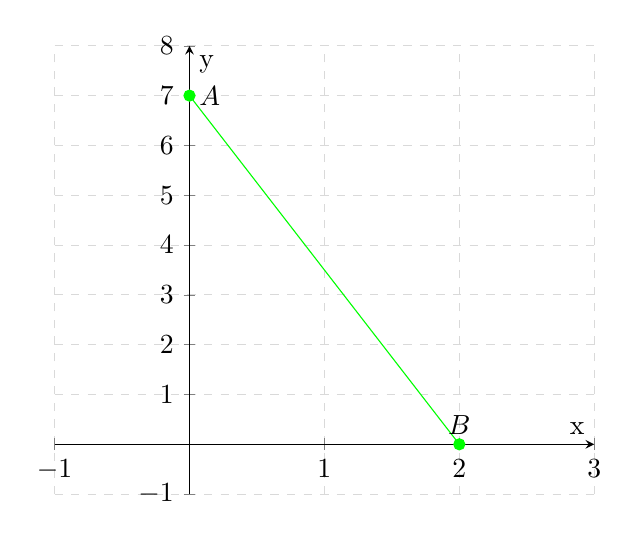
\begin{tikzpicture}
        \begin{axis}[
                xmin = -1,
                xmax = 3,
                ymin=-1,
                ymax=8,
                ytick={-1,0,1,2,3,4,5,6,7,8},
                xlabel=x,
                ylabel=y,
                grid=major,
                grid style = {dashed, gray!30},
                axis lines = center,
                clip = false
            ]

            \addplot[color=green,mark=*] coordinates {
                    (0, 7)
                    (2, 0)
                };
            \node [right] at (axis cs: 0, 7) {$A$};
            \node [above] at (axis cs: 2, 0) {$B$};
        \end{axis}
    \end{tikzpicture}
\end{center}
\begin{description}
    \item[a.] \begin{large}State the value of $c$.\end{large}
        $$c = 7$$
    \item[b.] \begin{large}Determine the slope of $AB$.\end{large}
        \marginpar[Note 1]{\raggedright The equation of a straight line is $y=mx+c$ %
            where $c$ = \textit{y-intercept}, $m$ = \textit{slope} and $x$ \& $y$ = \textit{x and y values}
        }
        Given the points
        $$
            \begin{array}{c}
                A \\
                \begin{pmatrix}
                    0 \ \ 7     \\
                    x_1 \ \ y_1 \\
                \end{pmatrix}
            \end{array}
            \begin{array}{c}
                B \\
                \begin{pmatrix}
                    2 \ \ 0     \\
                    x_2 \ \ y_2 \\
                \end{pmatrix}
            \end{array}
        $$

        and the slope($m$) of a straight line:

        $$
            m = \frac{y_2-y_1}{x_2-x_1}
        $$
        Substituting the values we get:
        $$
            \begin{aligned}
                m & = \frac{0-7}{2-0} \\
                m & = \frac{-7}{2}    \\
                m & = -3.5
            \end{aligned}
        $$

    \item[c.] \begin{large}Determine the mid-point of $AB$.\end{large}

        The midpoint of a straight line:

        $$
            m = (\frac{x_1+x_2}{2}, \frac{y_1+y_2}{2})
        $$
        Therefore substituting the values into the equation we get.

        $$
            \begin{aligned}
                m & = (\frac{0+2}{2}, \frac{7+2}{2}) \\
                m & = (1, 3.5)                       \\
            \end{aligned}
        $$
\end{description}

\section*{Question 2} \begin{large}A straight line joins two points H(-4, 6) and G(5, 3) .i.e\end{large}
$$
    \begin{array}{c}
        H \\
        \begin{pmatrix}
            -4 \ \ 6    \\
            x_1 \ \ y_1 \\
        \end{pmatrix}
    \end{array}
    \begin{array}{c}
        G \\
        \begin{pmatrix}
            5 \ \ 3     \\
            x_2 \ \ y_2 \\
        \end{pmatrix}
    \end{array}
$$
\begin{description}
    \item[a.] \begin{large}Calculate the slope of HG.\end{large}

        The slope of a straight line is
        $$
            m = \frac{y_2 - y_1}{x_2-x_1}
        $$
        Substituting the values given into the equation we get
        $$
            \begin{aligned}
                m & = \frac{3-6}{5-(-4)} \\
                m & = \frac{3-6}{5+4)}   \\
                m & = \frac{-3}{9}       \\
                m & = -\frac{1}{3}       \\
            \end{aligned}
        $$

    \item[b.] \begin{large}Determine the equation of HG.\end{large}

        The equation of straight line is
        $$
            y = mx + c
        $$
        Therefore choosing an ordered pair
        $$
            \begin{array}{c}
                H \\
                \begin{pmatrix}
                    -4 \ \ 6    \\
                    x_1 \ \ y_1 \\
                \end{pmatrix}
            \end{array}
        $$
        and substituting the values $m=-\frac{1}{3}$ into the $y=mx+c$ to find $c$ we get

        $$
            \begin{aligned}
                y & = mx + c                   \\
                6 & = -\frac{1}{3}(-4) + c     \\
                6 & = \frac{4}{3} + c          \\
                c & = 6 - \frac{4}{3}          \\
                c & = \frac{18}{3}-\frac{4}{3} \\
                c & = \frac{14}{3}             \\
            \end{aligned}
        $$

        Then substituting $m=-\frac{1}{3}$ and $c=\frac{14}{3}$ into the line equation we get

        $$
            y = -\frac{1}{3}x+\frac{14}{3}
        $$
        OR
        $$
            3y = -x + 14
        $$

    \item[c.] \begin{large}Write the slope of a line $\perp$ to HG.\end{large}

        Given that

        $$
            m_1 * m_2 = -1
        $$
        Substituting $m_1=-\frac{1}{3}$ we get

        $$
            \begin{aligned}
                -\frac{1}{3} * m_2 & = -1                     \\
                m_2                & = -1 \div -\frac{1}{3}   \\
                m_2                & = -1 \times -\frac{3}{1} \\
                m_2                & = 3                      \\
            \end{aligned}
        $$

    \item[d.] \begin{large}Determine the equation of the line which is $\perp$ to HG but passes through (7,2).\end{large}

        Given the equation of a line

        $$
            y = mx + c
        $$
        and $\perp$ line slope $m = 3$, $x = 7$ and $y=2$, we substitute the values into the line equation to get the y-intercept $c$

        $$
            \begin{aligned}
                y        & = mx + c \\
                mx + c   & = y      \\
                3(7) + c & = 2      \\
                21 + c   & = 2      \\
                c        & = 2 - 21 \\
                c        & = -19    \\
            \end{aligned}
        $$

        Therefore given than $m=3$ and $c=-19$ the line equation is

        $$
            \begin{aligned}
                y & = mx + c     \\
                y & = 3x + (-19) \\
                y & = 3x -19     \\
            \end{aligned}
        $$

    \item[e.] \begin{large}Determine the equation of a line PQ which is parallel to HG and passes through (-4,2).\end{large}

        Given the equation of the line HG is

        $$
            3y = -x + 14
        $$
        finding for the y-intercept $c$ and substituting the values $(-4, 2)$ we get

        $$
            \begin{aligned}
                3y   & = -x + c    \\
                3(2) & = -(-4) + c \\
                6    & = 4 + c     \\
                c    & = 2
            \end{aligned}
        $$
        therefore the equation of the line is
        $$
            3y = -x + 2
        $$

    \item[f.] \begin{large}Calculate the mid-point of HG.\end{large}

        Given the points
        $$
            \begin{array}{c}
                H \\
                \begin{pmatrix}
                    -4 \ \ 6    \\
                    x_1 \ \ y_1 \\
                \end{pmatrix}
            \end{array}
            \begin{array}{c}
                G \\
                \begin{pmatrix}
                    5 \ \ 3     \\
                    x_2 \ \ y_2 \\
                \end{pmatrix}
            \end{array}
        $$
        the midpoint of the is

        $$
            \begin{aligned}
                midpoint & = (\frac{x_1 + x_2}{2}, \frac{y_1+y_2}{2}) \\
                midpoint & = (\frac{-4 + 5}{2}, \frac{6+3}{2})        \\
                midpoint & = (\frac{1}{2}, \frac{9}{2})               \\
            \end{aligned}
        $$

    \item[g.] \begin{large}Calculate the length of the line HG.\end{large}

        The length of a line is

        $$
            \sqrt{(y_2-y_1)^2 + (x_2-x_1)^2}
        $$
        Therefore using the points

        $$
            \begin{array}{c}
                H \\
                \begin{pmatrix}
                    -4 \ \ 6    \\
                    x_1 \ \ y_1 \\
                \end{pmatrix}
            \end{array}
            \begin{array}{c}
                G \\
                \begin{pmatrix}
                    5 \ \ 3     \\
                    x_2 \ \ y_2 \\
                \end{pmatrix}
            \end{array}
        $$

        we get

        $$
            \begin{aligned}
                 & \sqrt{(3-6)^2 + (5-(-4))^2} \\
                 & \sqrt{(-3)^2 + (9)^2}       \\
                 & \sqrt{9 + 81}               \\
                 & \sqrt{90}                   \\
                 &\end{aligned}
        $$
        Therefore the length of the line HG is $9.487$ or `r sqrt(90)`.
\end{description}

\section*{Question 3}

\begin{description}
    \item[a.] \begin{Large}Given $y=5x+2$ and $-5x+y-3=0$, are these lines $\parallel$ , $\perp$ or neither?\end{Large}

        Writing both line equations in the form $y=mx+c$ we get:
        $$
            y = 5x + 2
        $$
        $$
            y = 5x + 3
        $$

        Therefore, given $m=5$ in both equations the lines are $\parallel$ to each other.

    \item[b.] \begin{Large} Given $3x+y=4$ and $x-3y+1=0$ are these lines $\parallel$, $\perp$  or neither?\end{Large}

        Writing both line equations in the form $y=mx+c$ we get:
        $$
            y = -3x+4
        $$
        $$
            y = \frac{1}{3}x + \frac{1}{3}
        $$
        Therefore $m_1=-3$ and $m_2=\frac{1}{3}$.
        A line is $\perp$ when $m_1 * m_2 = -1$.
        Checking to see if line is $\perp$.
        $$
            \begin{aligned}
                -3 \times \frac{1}{3} & = -\frac{3}{3} \\
                                      & = -1           \\
            \end{aligned}
        $$
        Therfore the lines are $\perp$.
\end{description}

\clearpage
\section*{\centering Homework}
\begin{Large} Find the midpoints, the length of the lines, the slopes and the equations of the straight lines passing through the points:\end{Large}
\begin{description}
    \item[1.]  \begin{Large} (-2, 10), (5, 3)\end{Large}

        \underline{MIDPOINT}
        $$
            \begin{aligned}
                midpoint & = (\frac{x_1+x_2}{2}, \frac{y_1+y_2}{2}) \\
                         & = (\frac{-2+5}{2}, \frac{10+3}{2})       \\
                         & = (\frac{3}{2}, \frac{13}{2})            \\
                         & = (1.5, 6.5)                             \\
            \end{aligned}
        $$

        \underline{LENGTH OF LINE}
        $$
            \begin{aligned}
                length \ of \ line & = \sqrt{(x_2-x_1)^2 + (y_2-y_1)^2} \\
                                   & = \sqrt{(5-(-2))^2 + (3-10)^2}     \\
                                   & = \sqrt{(7)^2 + (7)^2}             \\
                                   & = \sqrt{49 + 49}                   \\
                                   & = \sqrt{98}                        \\
                                   & = 9.90                             \\
            \end{aligned}
        $$

        \underline{SLOPE OF LINE}
        $$
            \begin{aligned}
                m & = \frac{y_2-y_1}{x_2-x_1} \\
                  & = \frac{3-10}{5-(-2)}     \\
                  & = -\frac{7}{7}            \\
                  & = -1                      \\
            \end{aligned}
        $$

        \underline{EQUATION OF THE LINE}

        Using the points $(-2, 10)$ and $m=1$ we find $c$
        $$
            \begin{aligned}
                y & = mx + c        \\
                c & = y - mx        \\
                c & = 10 - (-1)(-2) \\
                c & = 10 - 2        \\
                c & = 8             \\
            \end{aligned}
        $$
        Therefore the equation is
        $$
            y = -x + 8
        $$
        \begin{figure}[H]
            \begin{center}
                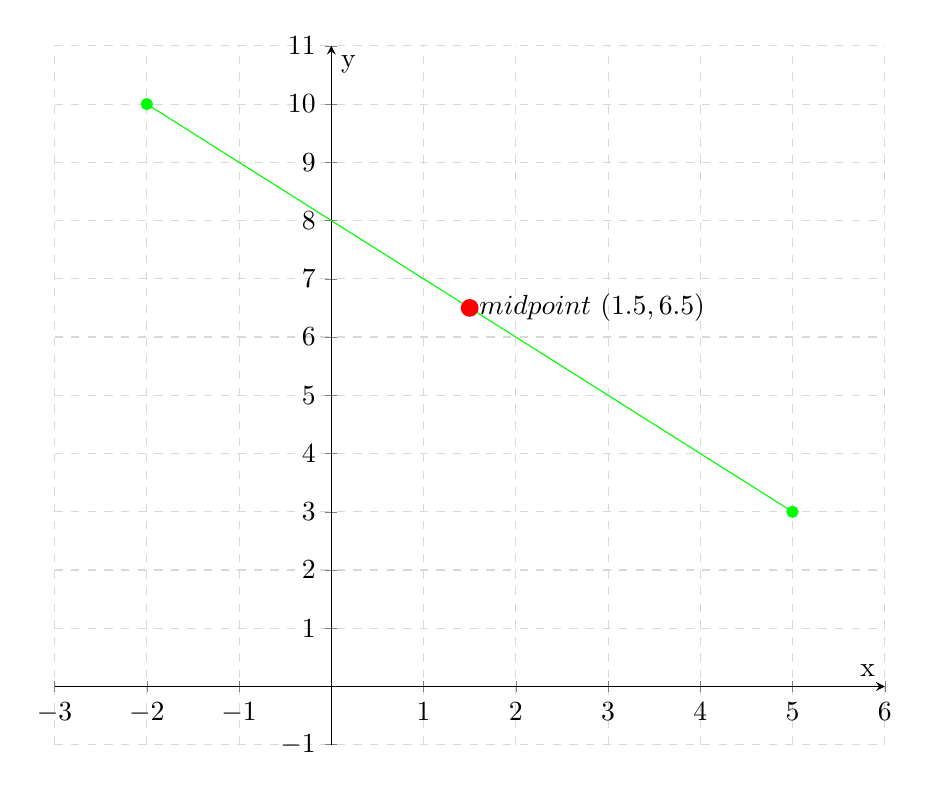
\begin{tikzpicture}
                    \begin{axis}[
                            width= \linewidth,
                            xmin = -3,
                            xmax = 6,
                            ymin=-1,
                            ymax=11,
                            ytick={-1,0,1,2,3,4,5,6,7,8,9, 10,11},
                            xlabel=x,
                            ylabel=y,
                            grid=major,
                            grid style = {dashed, gray!30},
                            axis lines = center,
                            clip = false
                        ]

                        \addplot[color=green,mark=*] coordinates {
                                (-2, 10)
                                (5, 3)
                            };

                        \addplot[color=red, mark=*, mark size=3pt] coordinates {
                                (1.5, 6.5)
                            };

                        \node [right] at (axis cs: 1.5, 6.5) {$midpoint \ (1.5, 6.5)$};

                    \end{axis}
                \end{tikzpicture}
                \caption{\label{Graph-2}Graph showing $y=-x+8$}
            \end{center}
        \end{figure}
        \clearpage
    \item[2.]  \begin{Large} (6, -2), (8, -3)\end{Large}

        \underline{MIDPOINT}
        $$
            \begin{aligned}
                midpoint & = (\frac{x_1+x_2}{2}, \frac{y_1+y_2}{2}) \\
                         & = (\frac{6+8}{2}, \frac{-2 + (-3)}{2})   \\
                         & = (\frac{14}{2}, \frac{-5}{2})           \\
                         & = (7, -2.5)                              \\
            \end{aligned}
        $$

        \underline{LENGTH OF LINE}
        $$
            \begin{aligned}
                length \ of \ line & = \sqrt{(x_2-x_1)^2 + (y_2-y_1)^2} \\
                                   & = \sqrt{8-6)^2 + (-3-(-2))^2}      \\
                                   & = \sqrt{(2)^2 + (-1)^2}            \\
                                   & = \sqrt{4 + 1}                     \\
                                   & = \sqrt{5}                         \\
                                   & = 2.24                             \\
            \end{aligned}
        $$

        \underline{SLOPE OF LINE}
        $$
            \begin{aligned}
                m & = \frac{y_2-y_1}{x_2-x_1} \\
                  & = \frac{-3-(-2)}{8-6}     \\
                  & = -\frac{1}{2}            \\
                  & = -0.5                    \\
            \end{aligned}
        $$

        \underline{EQUATION OF THE LINE}

        Using the points $(6, -2)$ and $m=-0.5$ we find $c$
        $$
            \begin{aligned}
                y & = mx + c         \\
                c & = y - mx         \\
                c & = -2 - (-0.5)(6) \\
                c & = -2 + 3         \\
                c & = 1              \\
            \end{aligned}
        $$
        Therefore the equation is
        $$
            y = -0.5x + 1
        $$
        \begin{figure}[H]
            \begin{center}
                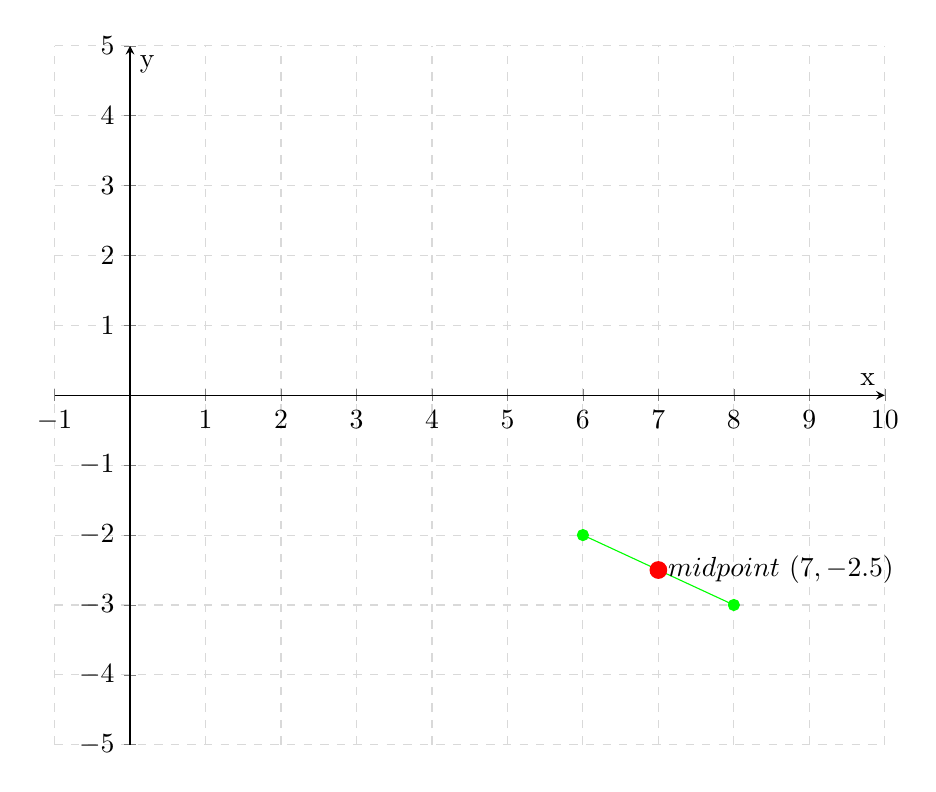
\begin{tikzpicture}
                    \begin{axis}[
                            width= \linewidth,
                            xmin = -1,
                            xmax = 10,
                            ymin=-5,
                            ymax=5,
                            ytick={-5, -4, -3, -2, -1, 0 ,1,2,3,4,5},
                            xlabel=x,
                            ylabel=y,
                            grid=major,
                            grid style = {dashed, gray!30},
                            axis lines = center,
                            clip = false
                        ]

                        \addplot[color=green,mark=*] coordinates {
                                (6, -2)
                                (8, -3)
                            };

                        \addplot[color=red, mark=*, mark size=3pt] coordinates {
                                (7, -2.5)
                            };

                        \node [right] at (axis cs: 7, -2.5) {$midpoint \ (7, -2.5)$};

                    \end{axis}
                \end{tikzpicture}
                \caption{\label{Graph-3}Graph showing $y=-0.5x+1$}
            \end{center}
        \end{figure}
        \clearpage
    \item[3.]  \begin{Large} (0, -6), (3, 0) \end{Large}

        \underline{MIDPOINT}
        $$
            \begin{aligned}
                midpoint & = (\frac{x_1+x_2}{2}, \frac{y_1+y_2}{2}) \\
                         & = (\frac{0+3}{2}, \frac{-6+0}{2})        \\
                         & = (\frac{3}{2}, \frac{-6}{2})            \\
                         & = (1.5, -3)                              \\
            \end{aligned}
        $$

        \underline{LENGTH OF LINE}
        $$
            \begin{aligned}
                length \ of \ line & = \sqrt{(x_2-x_1)^2 + (y_2-y_1)^2} \\
                                   & = \sqrt{3-0)^2 + (0-(-6))^2}       \\
                                   & = \sqrt{(3)^2 + (6)^2}             \\
                                   & = \sqrt{9 + 36}                    \\
                                   & = \sqrt{45}                        \\
                                   & = 6.71                             \\
            \end{aligned}
        $$

        \underline{SLOPE OF LINE}
        $$
            \begin{aligned}
                m & = \frac{y_2-y_1}{x_2-x_1} \\
                  & = \frac{0-(-6)}{3-0}      \\
                  & = -\frac{6}{3}            \\
                  & = 2                       \\
            \end{aligned}
        $$

        \underline{EQUATION OF THE LINE}

        Using the points $(0, -6)$ and $m=2$ we find $c$
        $$
            \begin{aligned}
                y & = mx + c        \\
                c & = y - mx        \\
                c & = (-6) - (2)(0) \\
                c & = - 6 - 0       \\
                c & = -6            \\
            \end{aligned}
        $$
        Therefore the equation is
        $$
            y = 2x - 6
        $$
        \begin{figure}[H]
            \begin{center}
                \begin{tikzpicture}
                    \begin{axis}[
                            width= \linewidth,
                            xmin = -1,
                            xmax = 5,
                            ymin= -7,
                            ymax= 1,
                            ytick={-7, -6, -5, -4, -3, -2, -1, 0 ,1},
                            xlabel=x,
                            ylabel=y,
                            grid=major,
                            grid style = {dashed, gray!30},
                            axis lines = center,
                            clip = false
                        ]

                        \addplot[color=green,mark=*] coordinates {
                                (0, -6)
                                (3, -0)
                            };

                        \addplot[color=red, mark=*, mark size=3pt] coordinates {
                                (1.5, -3)
                            };

                        \node [right] at (axis cs: 1.5, -3) {$midpoint \ (1.5, 3)$};

                    \end{axis}
                \end{tikzpicture}
                \caption{\label{Graph-4}Graph showing $y=2x-6$}
            \end{center}
        \end{figure}
        \clearpage
    \item[4.]  \begin{Large} (1, -7), (9, 0) \end{Large}

        \underline{MIDPOINT}
        $$
            \begin{aligned}
                midpoint & = (\frac{x_1+x_2}{2}, \frac{y_1+y_2}{2}) \\
                         & = (\frac{1+9}{2}, \frac{-7+0}{2})        \\
                         & = (\frac{10}{2}, \frac{-7}{2})           \\
                         & = (5, -3.5)                              \\
            \end{aligned}
        $$

        \underline{LENGTH OF LINE}
        $$
            \begin{aligned}
                length \ of \ line & = \sqrt{(x_2-x_1)^2 + (y_2-y_1)^2} \\
                                   & = \sqrt{(9-1)^2 + (0-(-7))^2}      \\
                                   & = \sqrt{(8)^2 + (7)^2}             \\
                                   & = \sqrt{64 + 49}                   \\
                                   & = \sqrt{113}                       \\
                                   & = 10.63                            \\
            \end{aligned}
        $$

        \underline{SLOPE OF LINE}
        $$
            \begin{aligned}
                m & = \frac{y_2-y_1}{x_2-x_1} \\
                  & = \frac{0-(-7)}{9-1}      \\
                  & = -\frac{7}{8}            \\
                  & = 0.88                    \\
            \end{aligned}
        $$

        \underline{EQUATION OF THE LINE}

        Using the points $(1, -7)$ and $m=0.88$ we find $c$
        $$
            \begin{aligned}
                y & = mx + c           \\
                c & = y - mx           \\
                c & = (-7) - (0.88)(1) \\
                c & = - 7 - 0.88       \\
                c & = -7.88            \\
            \end{aligned}
        $$
        Therefore the equation is
        $$
            y = 0.88x - 7.88
        $$
        \begin{figure}[H]
            \begin{center}
                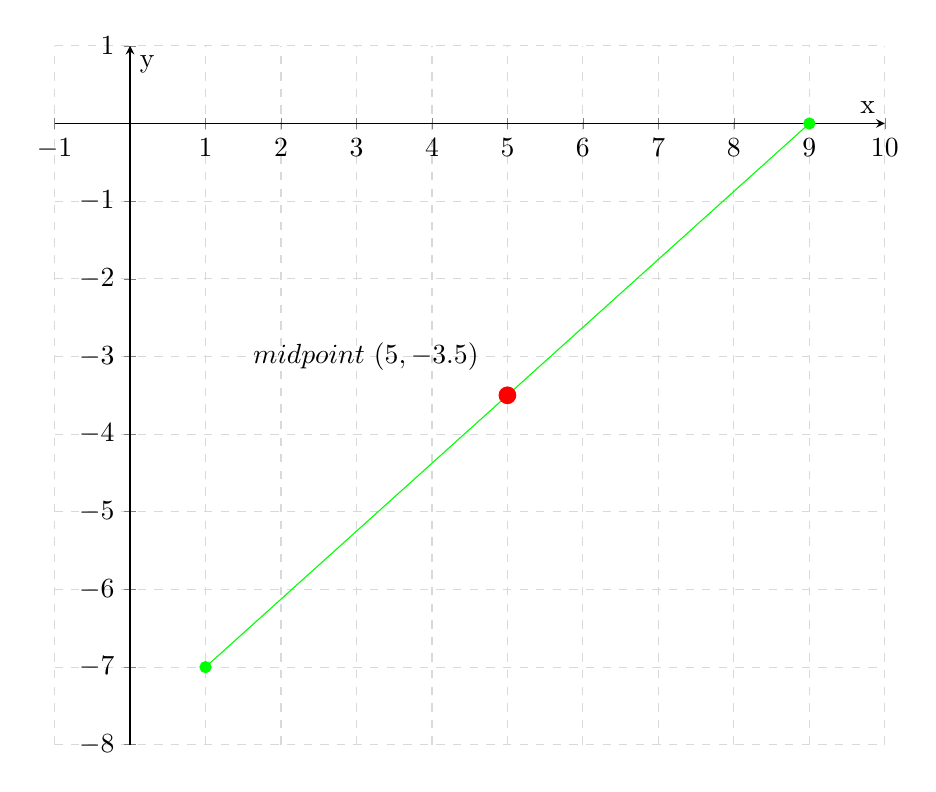
\begin{tikzpicture}
                    \begin{axis}[
                            width= \linewidth,
                            xmin = -1,
                            xmax = 10,
                            ymin= -8,
                            ymax= 1,
                            ytick={-8,-7, -6, -5, -4, -3, -2, -1, 0 ,1},
                            xlabel=x,
                            ylabel=y,
                            grid=major,
                            grid style = {dashed, gray!30},
                            axis lines = center,
                            clip = false
                        ]

                        \addplot[color=green,mark=*] coordinates {
                                (1, -7)
                                (9, 0)
                            };

                        \addplot[color=red, mark=*, mark size=3pt] coordinates {
                                (5, -3.5)
                            };

                        \node [right] at (axis cs: 1.5, -3) {$midpoint \ (5, -3.5)$};

                    \end{axis}
                \end{tikzpicture}
                \caption{\label{Graph-5}Graph showing $y=0.88x-7.88$}
            \end{center}
        \end{figure}
        \clearpage
\end{description}
\end{document}